\section{Methodology}

This section describes the software programs and libraries employed throughout the development of this project, as well as the hardware used to test the application created.

\subsection{Software}

\subsubsection{PX4 autopilot}
\label{subsec:px4}

PX4\footnote{\url{https://px4.io/}} is a widely-utilized autopilot flight stack designed for unmanned aerial vehicles (UAVs). Developed collaboratively by industry and academic experts, this open-source software benefits from an active global community, ensuring continuous improvements. It has been implemented in C++, a reliable and efficient programming language that gives it versatility and adaptability.

PX4 caters to various vehicle types, including racing drones, cargo drones, ground vehicles, and even submersibles. It accommodates both pre-built and custom-made drones, allowing developers to tailor their UAVs to specific requirements. Furthermore, PX4 supports integration with a range of sensors and peripherals, such as GPS, cameras, obstacle sensors, and more. This flexibility enhances UAV capabilities, ensuring efficient and safe operation in diverse environments.
PX4's significance extends within the Dronecode Project\footnote{\url{https://www.dronecode.org/}}, a comprehensive drone ecosystem. The Project includes essential components like the user-friendly QGroundControl ground station and the reliable Pixhawk hardware, known for its compatibility with PX4. The integration is further facilitated by the MAVSDK library, enabling seamless connections with companion computers, cameras, and additional hardware using the MAVLink protocol. This cohesive ecosystem empowers developers to leverage PX4's full potential and create innovative UAV solutions tailored to specific needs.

Central to PX4's functionality are its flight modes. These modes determine the autopilot's response to user commands and its management of autonomous flight. Offering various levels of assistance, flight modes simplify tasks like takeoff and landing while enabling precise control over flight trajectories and the maintenance of stable positions. PX4's adaptable flight modes ensure flexibility and reliability across a wide range of applications, from capturing aerial photographs to executing intricate autonomous missions.

In the context of this project, PX4 has played a pivotal role as the core component powering various aspects of the system. It serves as the heart of the simulation environment, replicating real-world flight conditions and interactions in a safe and cost-effective manner.
Moreover, PX4 acts as the key interface between the high-level commands generated by the developed application and the engine outputs required for precise control of the UAV. It effectively translates the intentions and directives of the application into concrete actions performed by the engines, propellers, and other flight control surfaces, while taking care of maintaining flight stabilization.
It implements sophisticated control algorithms and flight dynamics models to maintain stability, responsiveness, and safety during flight operations, thereby freeing the vision-based control application from focusing on low-level implementation.


\subsubsection{MAVLink and MAVSDK}
\label{subsec:mavlink}

MAVLink\footnote{\url{https://mavlink.io/en/}} is a lightweight messaging protocol designed as an integral part of the Dronecode Project.
In the context of a UAV driven by the PX4 autopilot, the MAVLink protocol plays a crucial role as a standardized communication framework. It enables seamless data exchange between the autopilot and various onboard components, allowing the transmission of telemetry data, commands, and status updates. MAVLink ensures interoperability and facilitates integration with custom-built or third-party components, enhancing the UAV's capabilities. By providing a reliable and efficient communication interface, MAVLink contributes to safe and coordinated flight operations, empowering developers to create sophisticated UAV systems with the PX4 autopilot at their core.

MAVSDK\footnote{\url{https://mavsdk.mavlink.io/main/en/index.html}}, on the other hand, is a cross-platform collection of libraries that enables seamless integration with MAVLink systems such as drones, cameras, and ground systems.
The library handles the underlying MAVLink messaging protocol, abstracting the complexity of message parsing and transmission. Developers can focus on the logic and commands they want to send to the autopilot without worrying about low-level communication details.
These libraries offer a user-friendly API for managing one or multiple vehicles, granting programmatic access to crucial vehicle information, telemetry, and control over missions, movements, and other operations. They can be utilized either onboard a drone's companion computer or on the ground via a ground station or mobile device, offering flexibility and convenience in system management.

While primarily implemented in C++, MAVSDK provides wrappers for Swift, Python, Java, and other languages. This project will employ the Python version of the library, allowing the developed application to send high-level commands and receive telemetry information from the autopilot without being concerned with the underlying MAVLink messages.


\subsubsection{QGroundControl}
\label{subsec:qgc}

QGroundControl\footnote{\url{http://qgroundcontrol.com/}} is an open-source ground control station developed by the Dronecode Project, serving as a crucial software component for managing and controlling MAVLink-enabled drones. Its intuitive interface and user-friendly design cater to both professionals and developers. QGroundControl seamlessly connects with PX4 Autopilot flight controllers via wired or wireless connections, facilitating communication with local simulators running the PX4 flight stack.

With QGroundControl, users can efficiently configure and calibrate their flight controllers to ensure optimal performance. It offers a streamlined approach to modifying and tracking configuration parameters, allowing for precise customization of drone systems. Additionally, QGroundControl allows sending essential flight commands such as arming, takeoff, and landing and grants precise control over the drone's movements.

One of the key features of QGroundControl is its map interface, which provides real-time GPS location visualization of the drone. Target waypoints can be defined on the map to plan flight missions, specifying desired speeds and altitudes for each location. This functionality enables the creation of automated flight paths and streamlines mission planning and execution. Figure \ref{fig:qgc-map} showcases the application interface on a Windows system.

\begin{figure}
  \centering
  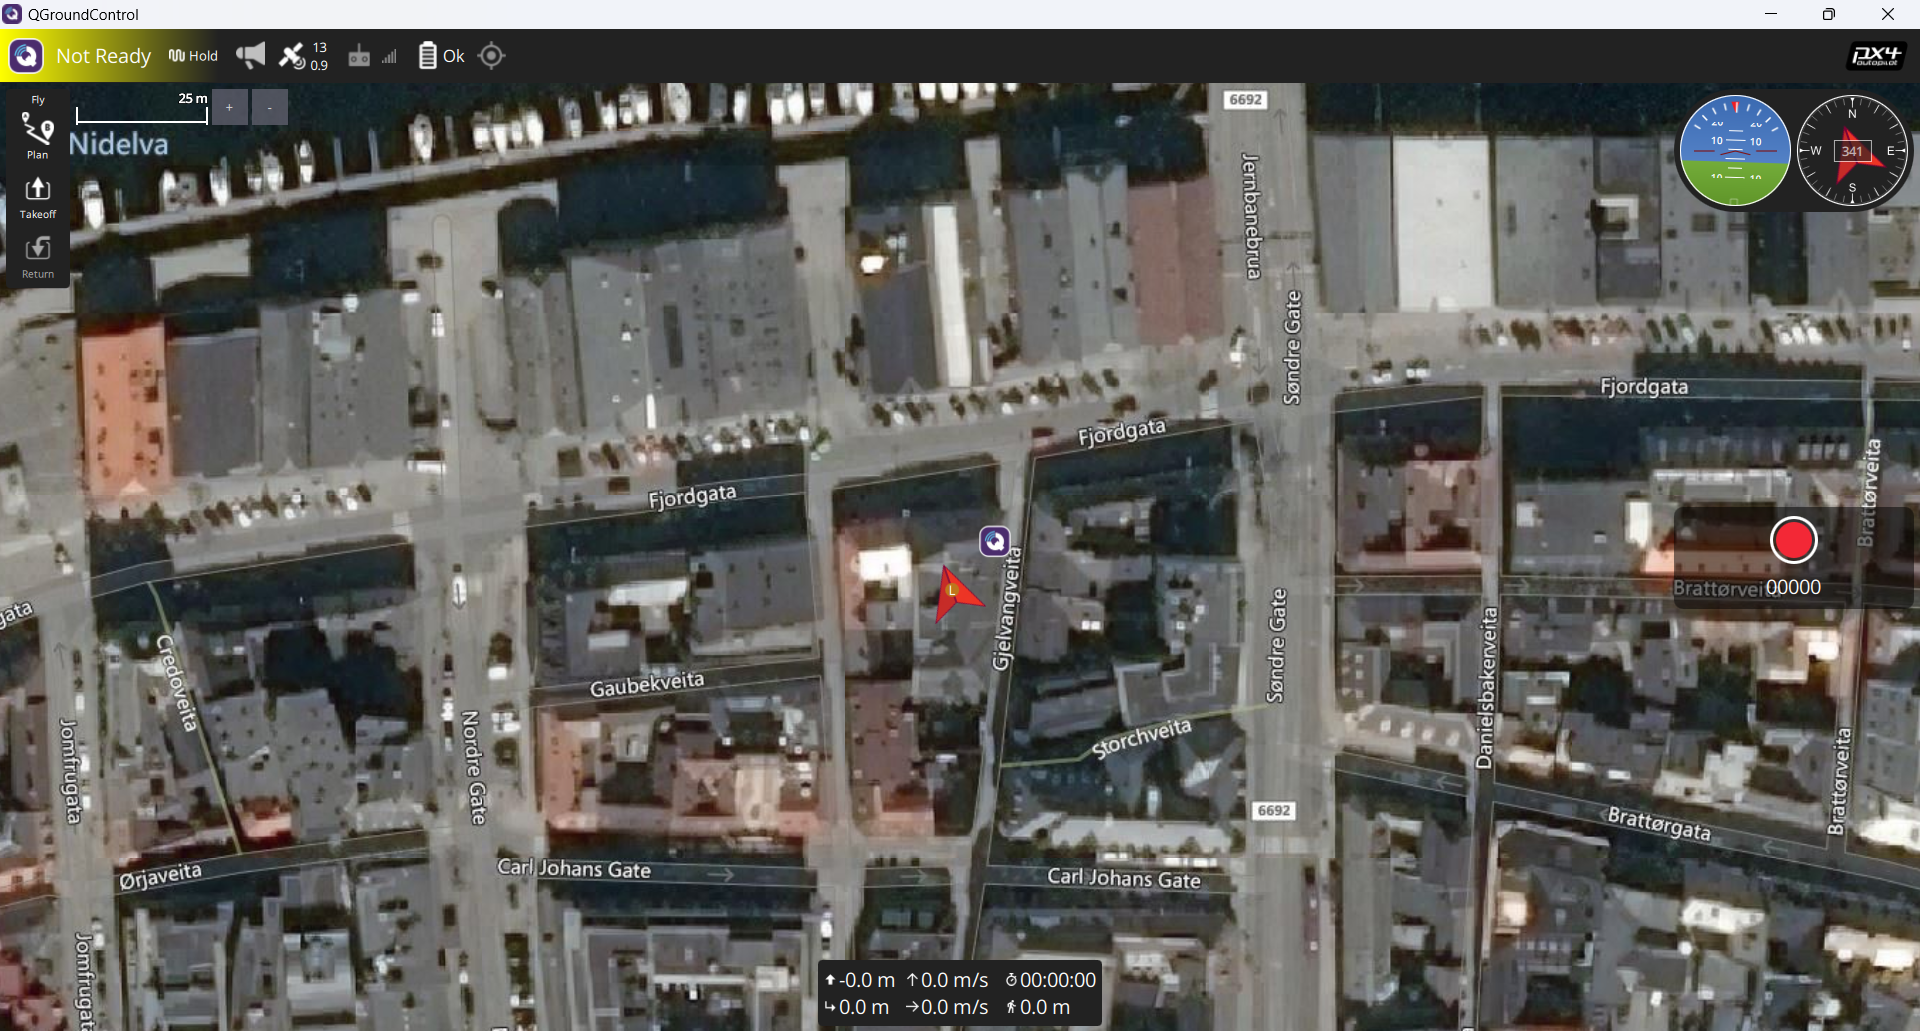
\includegraphics[width=\textwidth,keepaspectratio]{img/qgc-map.png}
  \caption{Main interface for the QGroundControl program.}
  \label{fig:qgc-map}
\end{figure}

\subsubsection{Unreal Engine and AirSim}
\label{subsec:unreal}

Unreal Engine\footnote{\url{https://www.unrealengine.com/en-US}} is a versatile 3D computer graphics tool primarily known for its game development capabilities. Initially introduced in 1998 for creating first-person shooters, the engine has evolved over time and is now widely used in various domains such as film, television, and research. It enables the creation of virtual sets, real-time rendering, computer-generated animation, and the development of virtual environments for architecture and vehicle design. Leveraging its real-time graphic generation capabilities, Unreal Engine serves as a powerful foundation for virtual reality applications. The interface of the engine, as shown in Figure \ref{fig:ue-interface}, provides a user-friendly environment for project development.

\begin{figure}
  \centering
  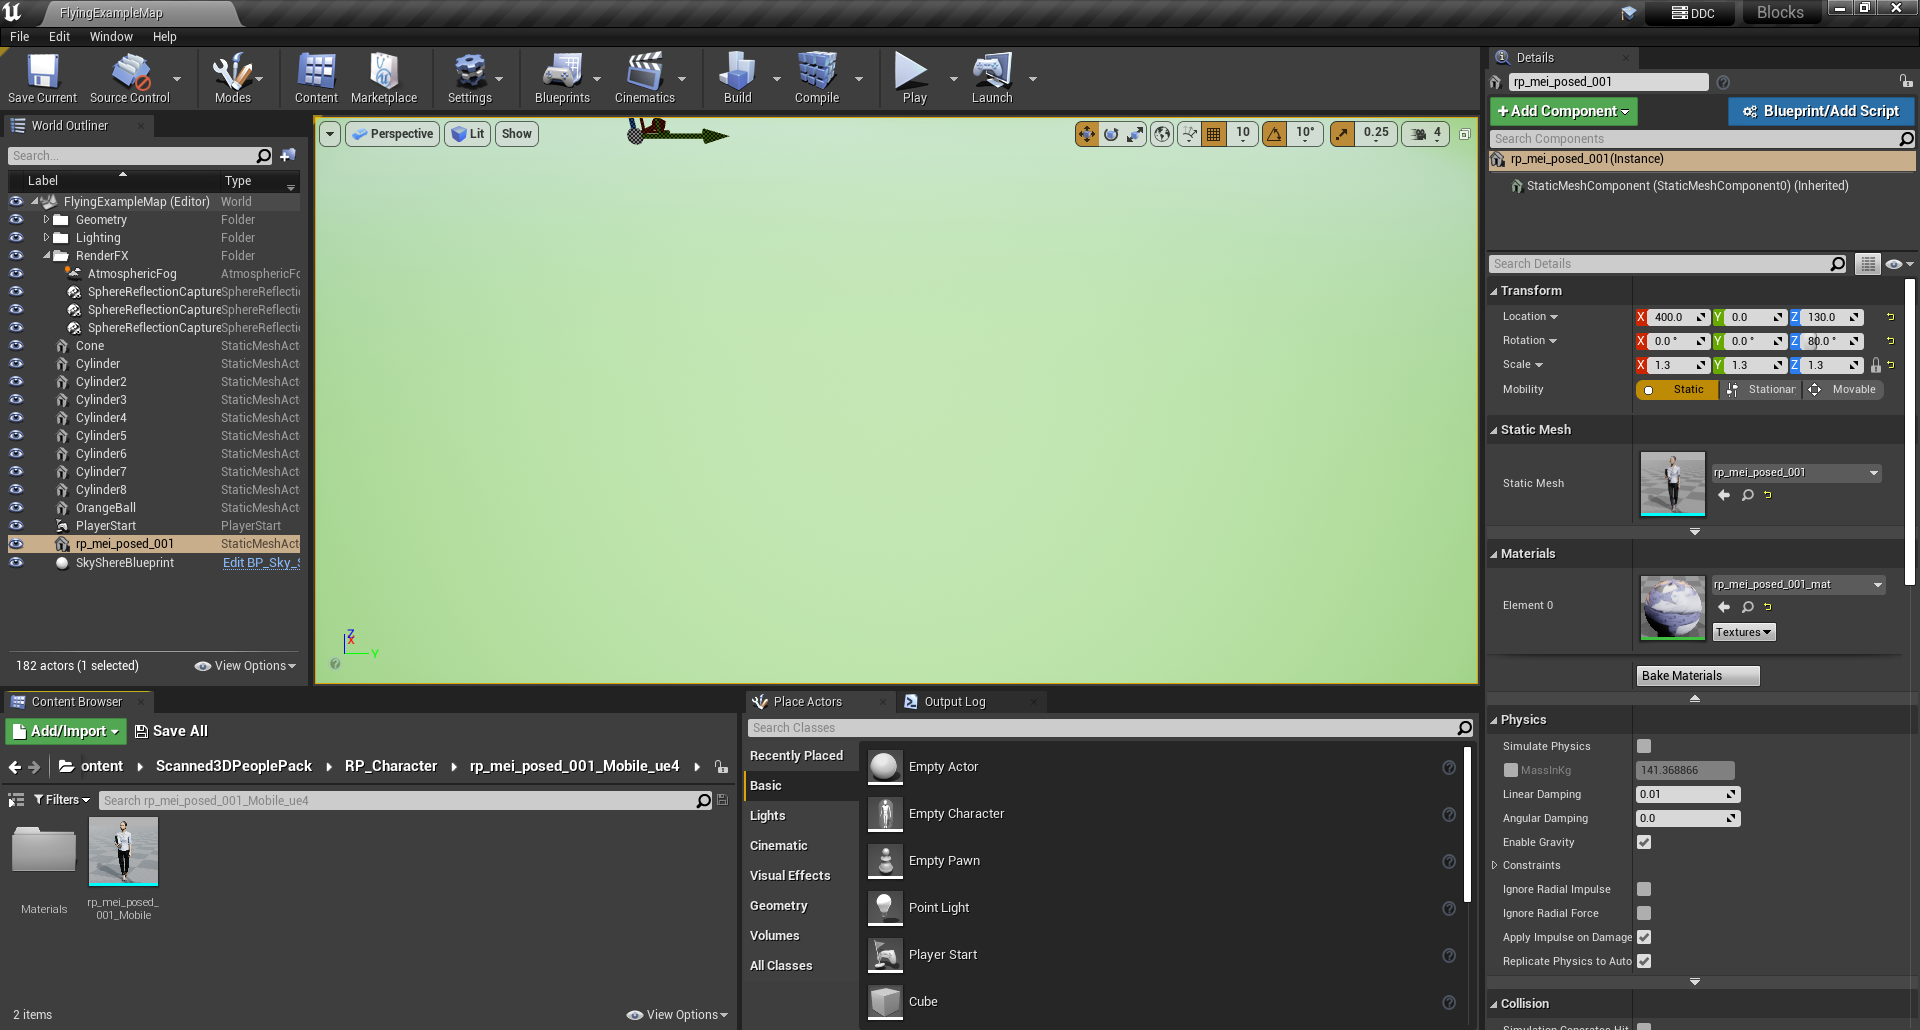
\includegraphics[width=\textwidth,keepaspectratio]{img/ue-interface.png}
  \caption{Project interface for the Unreal Engine.}\label{fig:ue-interface}
\end{figure}


AirSim\footnote{\url{https://microsoft.github.io/AirSim/}}, released by Microsoft in 2017, is an open-source simulator built on Unreal Engine. Designed for drones, cars, and other vehicles, AirSim supports both software-in-the-loop (SITL) and hardware-in-the-loop (HITL) simulations. It seamlessly integrates with popular flight controllers like PX4 and ArduPilot, allowing for realistic simulations that encompass both physical and visual aspects. Built as an Unreal Engine plugin, AirSim can be easily incorporated into existing Unreal environments. The main objective of AirSim is to provide a platform for AI research, facilitating experiments with deep learning, computer vision, and reinforcement learning algorithms for autonomous vehicles. To achieve this, AirSim offers the \texttt{airlib} library for data retrieval and vehicle control in a platform-independent manner. As of 2023, Microsoft has announced the development of a new simulation platform, Project AirSim, which will replace the original 2017 AirSim. While the original version will remain accessible to the public, it will no longer receive updates.

The combination of Unreal Engine and AirSim provides a robust framework for developing and testing autonomous systems. Researchers and developers can take advantage of the advanced capabilities of Unreal Engine to create visually immersive virtual environments, while AirSim's integration enables realistic simulations and AI experimentation. This integration offers a valuable toolset for exploring and advancing the field of autonomous vehicle technology.

AirSim plays a crucial role in this project by providing a simulated environment for testing and evaluating a vision-based control solution for tracking and following a person. By integrating AirSim into the project, the developed control algorithm can be applied to virtual drones within the simulated environment. This allows for comprehensive testing of the algorithms in various scenarios and conditions, providing valuable insights into its performance and effectiveness. Through this integration, the project benefits from the convenience and flexibility of simulation-based testing, ultimately leading to the development of a robust and reliable control solution for real-world deployment.


\subsubsection{MediaPipe}
\label{subsec:mediapipe}
MediaPipe\footnote{\url{https://google.github.io/mediapipe/}}, developed by Google, is an open-source project that provides customizable machine-learning solutions for live and streaming media. It offers a wide range of capabilities, including real-time perception of human pose, face landmarks, and hand tracking. These features enable the development of various applications, such as fitness and sports analysis, gesture control, sign language recognition, and augmented reality effects.

One of the key advantages of MediaPipe is its cross-platform support, allowing it to be used on Android, iOS, desktop/cloud, web, and IoT devices. It is designed to deliver accelerated processing and fast machine learning inference, even on less advanced hardware. This makes it accessible and applicable to a wide range of devices, ensuring that the developed solutions can be deployed on different platforms without sacrificing performance.
MediaPipe offers a flexible framework specifically tailored for complex perception pipelines, making it well-suited for tasks that require real-time analysis of visual data. 

Its versatility and robustness make it a valuable tool for researchers and developers working on computer vision and machine learning projects, empowering them to create innovative applications that leverage the power of streaming media, like the live feed from a camera onboard a drone.
Given the constraints of the onboard hardware for this project, which may have limited processing capabilities, Mediapipe's ability to perform on smaller devices becomes essential. Both the hand and human pose MediaPipe solutions will be used within this project to develop control mechanisms that react to the different positions detected (see Sections \ref{sec:hands} and \ref{sec:follow}).


\subsubsection{GitHub}
\label{subsec:github}

GitHub is an online hosting service that utilizes the Git version control system for software development. It serves as a centralized platform for storing code repositories, making it easy to manage and collaborate on projects. With a massive user base and millions of repositories, GitHub has become the leading source code host. 
In this project, both the software code\footnote{\url{https://github.com/l-gonz/tfg-giaa-dronecontrol}} and this report\footnote{\url{https://github.com/l-gonz/tfg-giaa-memoria}} are stored in GitHub. This allows for seamless version control and easy access to the project's codebase. 
Additionally, GitHub allows users to create static websites directly from repositories through GitHub Pages. This feature serves as an ideal solution for creating a landing or presentation page for the project. The project's website\footnote{\url{https://l-gonz.github.io/tfg-giaa-dronecontrol/}} contains an overview of the goals and implementation details, accompanied by videos showcasing the tests conducted in Chapter \ref{chap:validation}.


\subsubsection{OpenCV}
\label{subsec:opencv}

OpenCV is a widely used open-source library for computer vision, machine learning, and image processing, offering a rich collection of over 2000 algorithms. It provides powerful capabilities for various image-related tasks, such as capturing images or videos from cameras, extracting valuable information from them, and performing image editing operations.

Developed primarily in C++, OpenCV also offers Python wrappers, allowing users to leverage the flexibility and simplicity of Python while benefiting from the optimized performance of the underlying C++ code. OpenCV-Python integrates seamlessly with the Numpy library, which specializes in efficient numerical operations and adopts a MATLAB-like syntax. This integration enables smooth data exchange between OpenCV and other libraries, like Matplotlib, for convenient graph plotting.

In this project, the OpenCV and Numpy libraries play a crucial role in managing image data and facilitating communication with the MediaPipe library. They are utilized to process image information, illustrate detected landmarks, and enable the annotation of images within the DroneVisionControl application's graphical user interface. Additionally, Matplotlib has been employed to generate the graphs presented in Section \ref{sec:test-1-pid}. These libraries collectively contribute to the effective handling and analysis of image-related tasks throughout the project.

\subsection{Hardware}
\subsubsection{Pixhawk 4}
\label{subsec:pixhawk}

The Pixhawk 4 is an advanced autopilot module developed by Holybro\footnote{\url{https://shop.holybro.com/}} in collaboration with the Dronecode Project team. It is designed based on the open hardware design of the Pixhawk-project\footnote{\url{https://pixhawk.org/}} and optimized to run the PX4 flight stack on the NuttX\footnote{\url{https://nuttx.apache.org/}} operating system.

Equipped with an integrated accelerometer, gyroscope, magnetometer, and barometer, the Pixhawk 4 can autonomously control unmanned aerial vehicles using the native capabilities of the PX4 flight stack. These built-in sensors provide essential data for flight control and navigation.
These features make the Pixhawk 4 an integral component in the project's hardware setup.
Additionally, the Pixhawk 4 offers a range of connector sockets, depicted in Figure \ref{fig:pixhawk4}. The connectors allow for the expansion of its functionality with external sensors, input/output devices, or a companion computer. A companion computer is a separate computer connected to the flight controller to allow computationally expensive features like vision-based control. This project uses the Raspberry Pi 4 as the companion computer connected to the Pixhawk 4.


\begin{figure}[H]
  \centering
  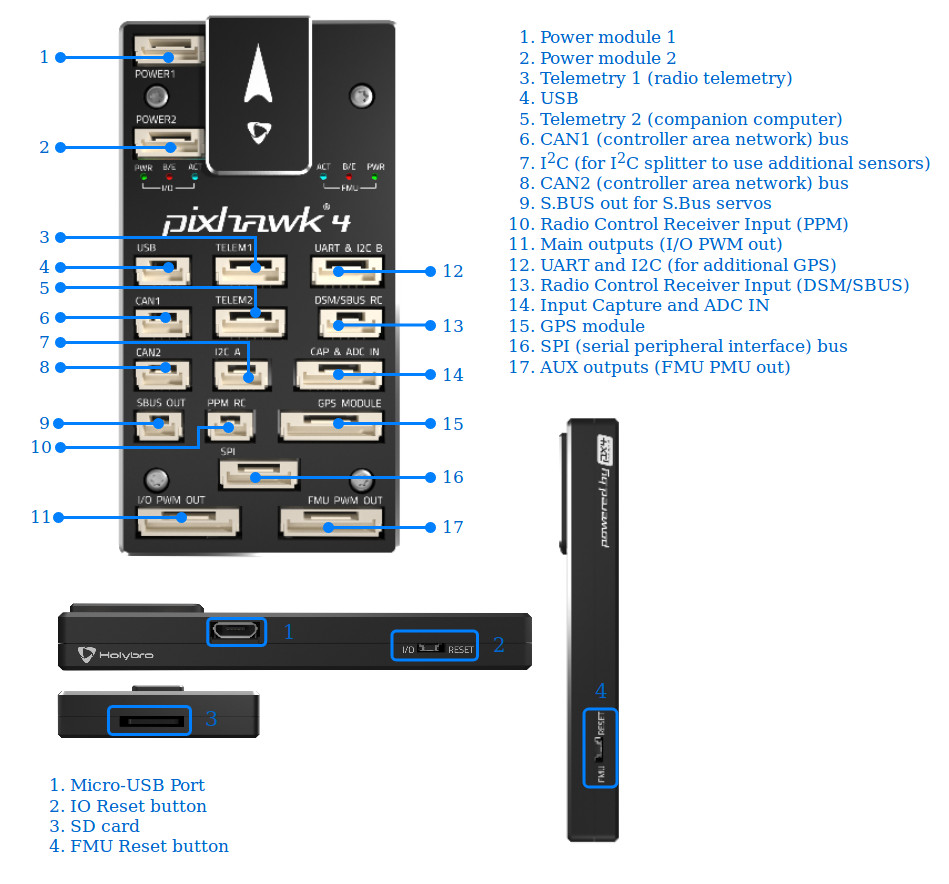
\includegraphics[width=0.6\textwidth,keepaspectratio]{img/pixhawk4.jpg}
  \caption{Side views and connector map for the Pixhawk 4 autopilot module.}
  \source{Adapted from \citetitle{px4-guide} \cite{px4-guide}.}
  \label{fig:pixhawk4}
\end{figure}

% The flight controller or autopilot is a circuit board equipped with sensors, and optimized for running the flight stack.
% The autopilot used in this project is the Pixhawk 4, designed by Holybro for the PX4 firmware.
% This board depends on a specific set of hardware components to function properly.
% These components include sensors, which collect environment data for processing, and actuators, which transform the output signals from the controller into movement.

% To determine the vehicle's state for stabilization and autonomous control, PX4 relies on sensors such as gyroscopes, accelerometers, magnetometers (compasses), and barometers.
% These are the sensors that are typically included already integrated with the autopilot's board.
% Additionally, a GPS or other positioning system is required to enable fully automatic flight modes and assisted features like altitude stabilization or mission planning.

% PX4 utilises outputs to control motor speed, flight surfaces (e.g., ailerons and flaps), camera triggers, parachutes, grippers, and other payloads. Brushless motors, controlled by Electronic Speed Controllers (ESCs) connected to the flight controller, rotate the propellers in most PX4 drones. These drones typically employ Lithium-Polymer (LiPo) batteries, which are connected to the system using a Power Module or Power Management Board, providing separate power for the flight controller and ESCs. 

% For manual control of the vehicle, a \acrfull{rc} system is employed, consisting of a remote control unit that communicates stick and control positions to a receiver on the vehicle. Advanced RC systems can also receive telemetry information from the autopilot, providing feedback to the operator. Telemetry radios offer an alternative means of communication with the autopilot, establishing a wireless MAVLink connection between a ground control station and a PX4-powered vehicle. This enables real-time parameter tuning, flight mode commands, telemetry inspection, and on-the-fly mission changes.

% In an actual UAV, the PX4 software runs on dedicated hardware like the Pixhawk 4 mentioned. This hardware includes all the essential sensors for flight as well as interfaces to connect additional actuators and I/O systems (RC, telemetry radio). 
% However, on a simulated environment like the one described in Section \ref{sec:devenv}, all the hardware components of the sensors and actuators are simulated on the same computer running the flight stack.


\subsubsection{Raspberry Pi 4B}
\label{subsec:rpi}

The Raspberry Pi is a series of single-board computers known for their affordability, compact size, and user-friendly design. The Raspberry Pi Model 4B\footnote{\url{https://www.raspberrypi.com/products/raspberry-pi-4-model-b/}}, used in this project, offers improved performance, expanded video output capabilities, and enhanced peripheral connectivity compared to previous models. Despite these advancements, it maintains the same affordable price and compact form factor.

The Raspberry Pi 4B computer comes as a bare circuit board without any additional components like a housing or cooling fan, as shown in Figure \ref{fig:rpi4b}. It features various ports, including USB, HDMI, and Ethernet, as well as built-in Wi-Fi and Bluetooth connectivity. Additionally, it provides a 40-pin GPIO (General Purpose Input/Output) header, allowing direct connection of external devices for expanded functionality.
The Raspberry Pi runs the Raspbian OS, a free operating system based on Debian that is specifically optimized for Raspberry Pi hardware. However, it is also compatible with other Linux distributions, which offers flexibility in software choices.

By leveraging the Raspberry Pi 4B as a companion computer to the Pixhawk 4 board, computationally intensive computer vision tasks are offloaded to a dedicated processor. Thanks to its compact size, it can be integrated onboard the vehicle to facilitate real-time processing of a camera feed from an attached camera. This setup enhances the capabilities of the system by leveraging the Raspberry Pi's processing power for efficient and responsive image analysis during flight operations.

\begin{figure}[H]
  \centering
  \includegraphics[width=0.5\textwidth,keepaspectratio]{img/rpi4b.jpg}
  \caption{Raspberry Pi 4 Model B}
  \source{Wikimedia Commons \cite{rpi4-side}.}
  \label{fig:rpi4b}
\end{figure}


\subsubsection{Holybro X500}
\label{subsec:x500}

The Holybro X500\footnote{\url{https://docs.px4.io/main/en/frames_multicopter/holybro_x500_pixhawk4.html}} is a quadcopter specifically designed by Holybro to be compatible with the PX4 autopilot system. It is supplied as a comprehensive development kit that consists of essential components for assembly. These components include a durable carbon-fibre twill frame, the Pixhawk 4 flight controller, a power management board, four motors, a GPS module, an RC receiver, and a telemetry radio. The kit does not include a camera for computer vision applications, but the frame leaves some space to add one for this project (see Section \label{subsec:onboard}). The kit is designed for easy assembly, with a build time of approximately 3 hours and no need for specialized tools. The completed quadcopter is depicted in Figure \ref{fig:x500}, showcasing the outcome of the assembly process.

\begin{figure}[H]
  \centering
  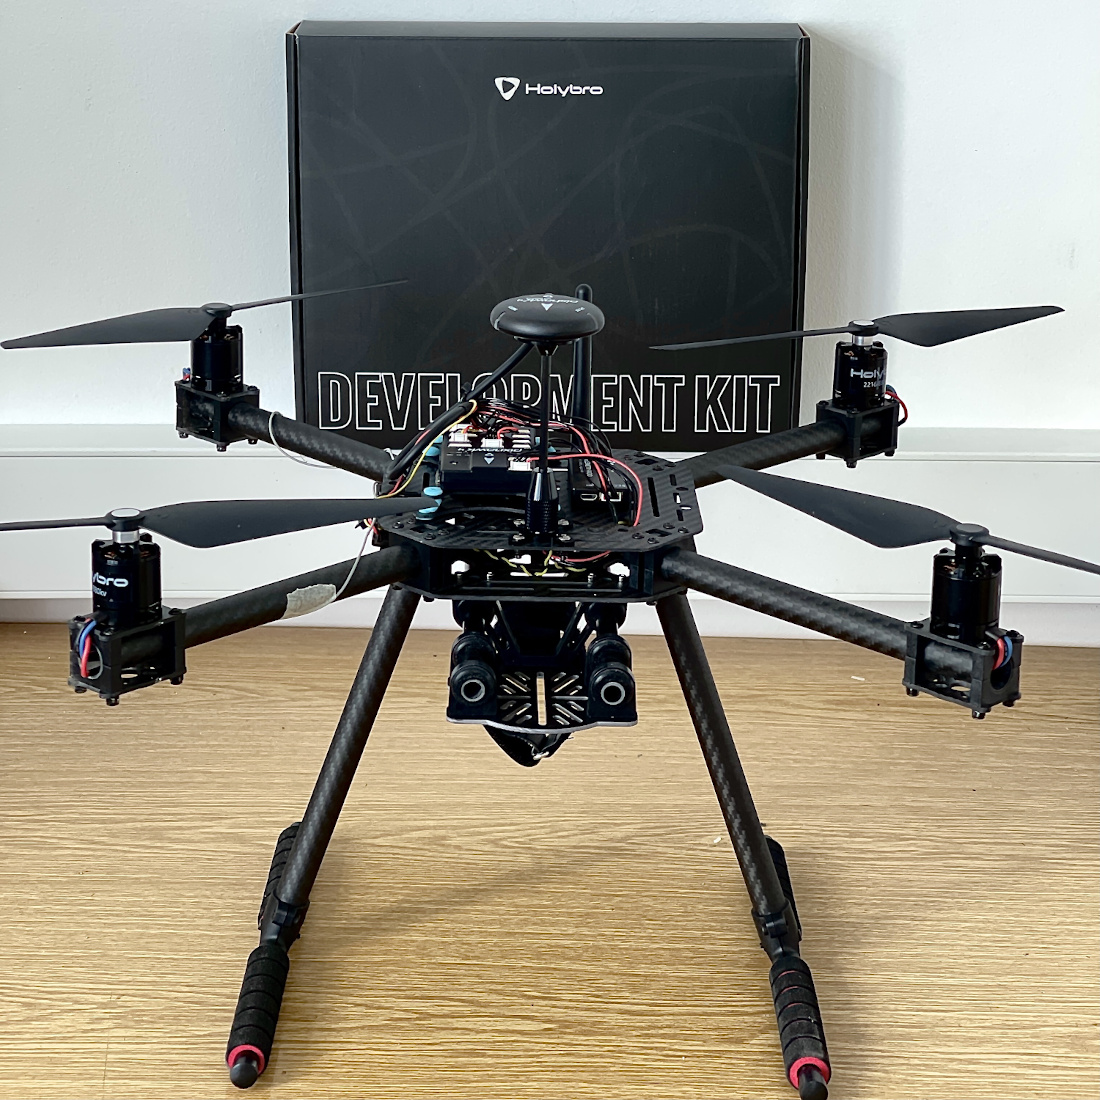
\includegraphics[width=0.5\textwidth,keepaspectratio]{img/X500-assembled.jpg}
  \caption{Fully assembled X500 kit.}
  \source{Adapted from \citetitle{px4-guide} \cite{px4-guide}.}
  \label{fig:x500}
\end{figure}

\subsubsection{Logitech C920 camera}
\label{subsec:camera}

The chosen camera to add to the vehicle frame to support vision-based control features during flight is the Logitech C920 1080p webcamera\footnote{\url{https://www.logitech.com/en-gb/products/webcams/c920-pro-hd-webcam.960-001055.html}}. This camera offers a field of view of 78º, 1080p resolution at 30 frames per second and autofocus while weighing 162 grams. In practice, any camera with a contained weight and size that offers enough quality for the pose detection library to function correctly can be used to obtain similar results for this project.